\documentclass[aspectratio=169]{beamer}
\usepackage{xcolor}
\usepackage{amsmath, amssymb}
\usepackage{booktabs}
\usepackage{multirow}

\AtBeginSection[]{
  \begin{frame}
  \vfill
  \centering
  \begin{beamercolorbox}[sep=8pt,center,shadow=true,rounded=true]{title}
    \usebeamerfont{title}\insertsectionhead\par%
  \end{beamercolorbox}
  \vfill
  \end{frame}
}

%Information to be included in the title page:
\title{Fiscal stimulus policies according to HANK-SAM}
\author{Tobias Broer \and Jeppe Druedahl \and  Karl Harmenberg \and Erik \"{O}berg}
\institute{Paris School of Economics, University of Copenhagen,\\ University of Oslo, Uppsala University}
\date{September 2023}

\begin{document}

\frame{\titlepage}

\begin{frame}{Research question and approach}
\label{slide:research_question}
\begin{block}{Research question}
    Which fiscal policies are most cost effective in stabilizing unemployment?
\end{block}


\begin{block}{Motivation}
Resurgence of countercyclical fiscal policies as stabilization tool
\begin{itemize}
    \item Government: expenditures
    \item Households: cash transfers + UI increases and extensions
    \item Firms: retention and hiring subsidies
\end{itemize}
\end{block}

\begin{block}{Approach}
    Compute fiscal multipliers for different fiscal policies in an equilibrium model with empirically grounded interaction between firm hiring-and-firing decisions and consumption-saving decisions of households. 
\end{block}


\end{frame}

\begin{frame}{Literature}
	\footnotesize	
	\begin{block}{Fiscal multipliers in HANK}
		Kaplan et al. (2018), Hagedorn et al. (2019), Alves et al. (2020), Carroll et al. (2023)
	\end{block}
	
	\medskip
	
	\begin{block}{HANK-SAM}
		Gornemann et al.(2016), Den Haan et al. (2018), Challe (2020), McKay-Reis (2020), Ravn-Sterk (2021), Bilbiie (2021), Cho (2022), Graves (2022), Kekre (2022).
	\end{block}

\label{slide:literature}

\medskip
\scriptsize
\textbf{SAM (inelastic entry):}
Coles-Kelishomi (2018), Fujita-Ramey (2007), Haefke-Reiter (2020),
Leduc-Liu (2020), Mercan et al. (2021), Engbom (2021).

\smallskip

%\textbf{SAM (endogenous separations): } Mortensen-Pissarides (1994), Den Haan et al. (2000), Shimer (2012), Fujita-Ramey (2012), Barnichon (2012), Trigari (2019).

\smallskip

\textbf{RANK-SAM:}
Walsh (2005), Gertler et al. (2008), Trigari (2009), Gali (2010),
Ravenna-Walsh (2012), Christiano et al. (2016).

\smallskip

\textbf{Consumption effects
of unemployment (risk): }Gruber (1997), Aguiar-Hurst
(2005), Eusepi-Preston (2015), Chodorow-Reich-Karabarbounis (2016),
Kolsrud et al. (2018), Harmenberg-\"{O}berg (2021), Graves (2022), Ganong-Noel
(2019), Ganong et al. (2022).

\bigskip

\normalsize
\textbf{This paper:}
Quantitative framework for consumer- \emph{and} firm-side fiscal stimulus:

\hspace{2mm}1. Realistic degree of partial insurance

\hspace{2mm}2. Realistic hiring-and-firing dynamics

\end{frame}

\section{Model}

\begin{frame}{Model overview}
    \begin{itemize}
        \item[HA] Households facing incomplete markets and endogenous income risk due to time-varying unemployment risk
        \begin{itemize}
            \item Government finances unemployment insurance and other expenditures through taxes and debt issuance
        \end{itemize}
        \item[NK]  Central bank with inflation-targeting Taylor rule, intermediate-goods producers giving rise to a Phillips curve
        \item[SAM] Frictional labor market with endogenous separations + sluggish vacancy creation
    \end{itemize}
\end{frame}

\begin{frame}{HA block: labor income}

\begin{block}{Labor income process}
A worker either receives wage $W$, high replacement rate $\color{blue}\overline{\phi}_t$, or low replacement rate $\underline{\phi}$. 
\begin{itemize}
	\item[Wage] A worker earns the wage $W$ if employed
	\item[SAM] A worker loses her job with probability $\delta_t$, an unemployed worker finds a new job with probability $\lambda_{it}^{u}=\lambda^u_t s(u_{i,t-1})$; exogenous search intensity $s(\cdot)$ is declining in unemployment duration
	\item[UI] Unemployment benefits are duration dependent, the worker receives replacement rate $\color{blue}\overline{\phi}_t$ for the first $\color{blue}\overline{u}_t$ months, and subsequently $\underline{\phi}$; with probability $\pi^\text{UI}$, the worker only receives replacement rate $\underline{\phi}$ (limited uptake)
\end{itemize}

\end{block}
\bigskip
\footnotesize {\color{blue} blue} denotes fiscal-policy variables
\end{frame}

\begin{frame}{HA block: household problem}
Workers consume income hand-to-mouth ($\beta_i=0$), or self-insure against unemployment risk by accumulating government bonds ($\beta_i>0$). Both types of workers face the same income process.
\bigskip
\begin{block}{Value function (self-insuring worker)}
The worker's value function is given by
\begin{align*}
	V_{t}^{w}(u_{it},a_{it-1})=&	\max_{c_{it},a_{it}}\frac{c_{it}^{1-\sigma}}{1-\sigma}+\beta_i\underline{V}_{t+1}^{w}\left(u_{it},a_{it}\right),\\
\text{{s.t.} }&	a_{it}+c_{it}=R_{t}^{\text{real}}a_{it-1}+(1-\tau_{t})y_{t}(u_{it})+Div_{t}+{\color{blue}T_t}.\\
	&a_{it}\geq0.
\end{align*}
The worker receives labor income net of taxes $(1-\tau_t)y_t(u_{it})$, dividends from firm ownership $Div_t$, and (potentially) a transfer from the government $\color{blue}T_t$.
\end{block}

\end{frame}

\begin{frame}{HA block: government}
\begin{itemize}
	\item The government raises taxes, issues bonds and spends funds on unemployment insurance, government consumption, universal transfers to all households, retention subsidies to matched firms, and hiring subsidies to newly formed matches.
	\item Long-term bonds: one unit of government bonds is a promise to a sequence of geometrically decaying coupon payments, paying out $\delta_{q}^{k-1}$ units of consumption $k$ periods into the future.
\end{itemize}

\end{frame}

\begin{frame}{SAM block}
	\begin{block}{Separation decision}
		A firm must pay continuation cost $\chi\sim G$ $\Rightarrow$ cutoff $\chi_{c,t}$. Resulting Bellman equation:
	\begin{align*}
		V_{t}^{j}	=P_{t}^{X}Z_{t}-W+\text{\color{blue}retention subsidy}_{t}+\beta^{\text{firm}}\mathbb{E}_{t}\left[\int^{\chi_{c,t+1}}(V_{t+1}^{j}-\chi_{t+1})dG(\chi_{t+1})\right].
	\end{align*}
	Functional-form assumption on $G$: $\delta_{t}=\delta_{ss}\left(\frac{V_{t}^{j}}{V_{ss}^{j}}\right)^{-{\color{red}\psi}}$.
	\end{block}

	\begin{block}{Vacancy-creation decision}
	Mass $F$ of entrants draw entry cost $c\sim H$. Bellman equation for vacancy value:
		\begin{align*}
 			V_{t}^{v}=-\kappa+\lambda_{t}^{v}(V_{t}^{j}+\text{\color{blue}hiring subsidy}_{t})+(1-\lambda_{t}^{v})(1-\delta_{ss})\beta^{\text{firm}}\mathbb{E}_{t}[V_{t+1}^{v}].
 		\end{align*}
 Functional-form assumption on $H$: entrants $\iota_{t}=\iota_{ss}\left(\frac{V_{t}^{v}}{V_{ss}^{v}}\right)^{\color{red}\xi}.$
	\end{block}

\medskip
Key parameters: elasticities $\color{red} \psi, \xi$ of separations and vacancy creation
\end{frame}

\section{Model mechanism}

\begin{frame}{Model mechanism}
	\begin{itemize}
		\item One simplifying assumption: Profits are consumed by hand-to-mouth capitalists \\ ($\leadsto$ profits from NK and SAM blocks do not enter HA block)
		\item With these assumptions, the three blocks interact in a transparent manner \\ $\leadsto$ can summarize model with flow chart (``directed graph'') \\ $\leadsto$ propositions \\ $\leadsto$ heuristics for interpreting the quantitative results
	\end{itemize}
\end{frame}

\begin{frame}{Model overview -- under profit assumption}
\begin{center}
    \includegraphics<1-3>[scale=0.6]{figs/model_diagram_2.pdf}
    \includegraphics<4->[scale=0.6]{figs/model_diagram_2.pdf}
\end{center}
\begin{onlyenv}<1>
\begin{block}{Sequence-space Jacobian summary of model} 
The model is summarized by three linear operators $M_\text{HA}$, $M_\text{NK}$ and $M_\text{SAM}$:
\begin{align*}
    \mathbf{s} = M_\text{SAM}(\mathbf{p^x}+\mathbf{z}), && \mathbf{r^\text{real}} = M_\text{HA} \mathbf{s}, &&\mathbf{p^x} = M_\text{NK} \mathbf{r^\text{real}}.
\end{align*}
Boldface: vectors of paths, $\mathbf{x}=[x_0,x_1, \ldots]$. Note: not a DAG, cyclical feedback loop.
\end{block}
\end{onlyenv}
\begin{onlyenv}<2>
\begin{block}{Proposition (unemployment response to a productivity shock)} 
    The response of unemployment is given by 
    \begin{align*}
        \mathbf{u} = M_u(I-M_\text{SAM}M_\text{NK}M_\text{HA})^{-1}M_\text{SAM} \mathbf{z}
    \end{align*}
     where $M_u$ is given by the relation $\mathbf{u} = M_u\mathbf{s}$.
    \end{block}
\end{onlyenv}
\begin{onlyenv}<3>
    \begin{block}{Proposition (unemployment response to a government-expenditure shock)} 
        The response of unemployment is given by 
        \begin{align*}
            \mathbf{u} = M_u(I-M_\text{SAM}M_\text{NK}M_\text{HA})^{-1}M_\text{SAM}M_\text{NK}M_g \mathbf{g}
        \end{align*}
        where $M_g$ is the partial-equilibrium response of the real interest rate to $\mathbf{g}$.
        \end{block}
    \end{onlyenv}
\begin{onlyenv}<4>
        \begin{block}{Heuristics for quantitative policy evaluation} 
            \begin{itemize}
                \item The comparison of demand-side (HA) policies is insensitive to $M_\text{NK}$, $M_\text{SAM}$.
                \item The comparison of supply-side (SAM) policies is insensitive to $M_\text{HA}$, $M_\text{NK}$.
                \item The comparison of demand-side vs. supply-side policies depends on all blocks (including $M_\text{NK}$)
            \end{itemize}
        \end{block}
\end{onlyenv}
\end{frame}

\section{Calibration}
\begin{frame}{Calibration: key targets}
	\label{slide:calibration}
    \begin{block}{Heterogeneous-agent block}
        Match (i) consumption drop upon unemployment and (ii) upon unemployment-benefits expiration.
        \begin{itemize}
            \item MPC untargeted but reasonable (0.41 quarterly)
        \end{itemize}
        \hyperlink{slide:ui}{\beamerbutton{unemployment insurance}}
        \hyperlink{slide:preferences}{\beamerbutton{consumption profile upon unemployment}}
        \hyperlink{slide:rel_job_finding}{\beamerbutton{duration-dependent job-finding rate}}
    \end{block}

    \begin{block}{Search-and-matching block}
        Match aggregate facts on (i) the contribution of separation rate and job-finding rate to unemployment dynamics and (ii) that separations lead the job-finding rate \textit{with} the elasticities of separations and vacancies to profitability.
        \begin{itemize}
            \item Data in favor of departure from standard DMP model: low elasticity of vacancy creation, positive elasticity of separations.
        \end{itemize}
    \end{block}
    \hyperlink{slide:dyn_job_finding_seprations}{\beamerbutton{dynamics of job-finding rate and separations}}

    \bigskip

    New-Keynesian block: standard values

\end{frame}

\begin{frame}{Comparison with RA and standard DMP}
	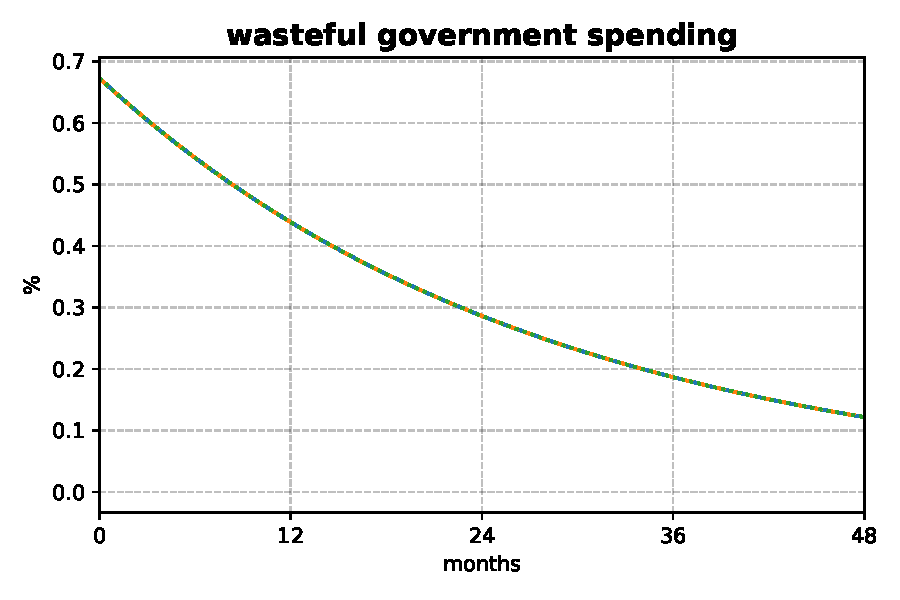
\includegraphics[scale=0.45]{results/IRF_G_compare_titled.pdf}
    \hfill
    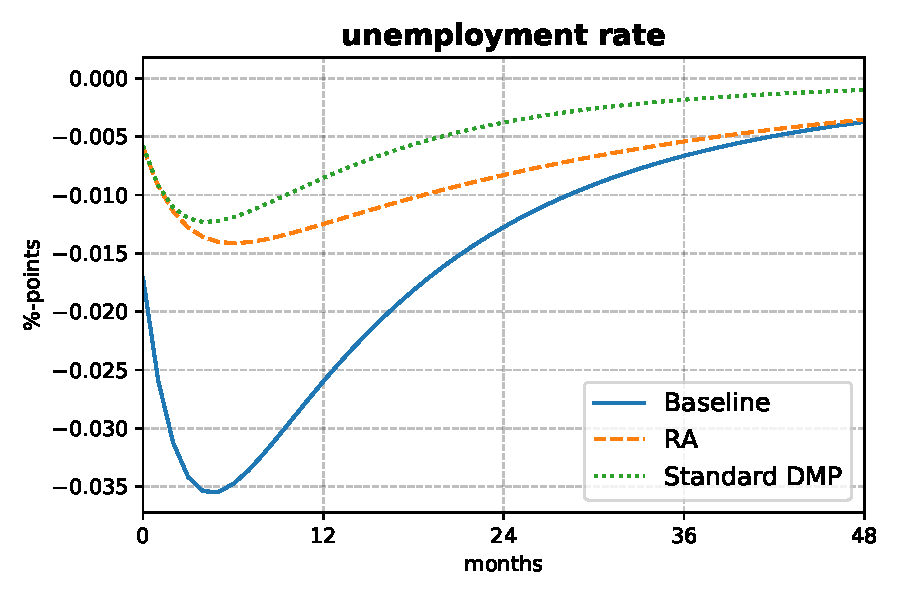
\includegraphics[scale=0.45]{results/IRF_u_compare_titled.pdf}

\begin{itemize}
	\item RA: replace heterogeneous-agent block with a representative agent
	\item Standard DMP: replace our labor-market calibration with standard DMP calibration (exogenous separations, infinitely elastic vacancy creation)
	\item Both the calibrated HA block and the calibrated SAM block amplify fiscal multipliers
\end{itemize}
\end{frame}



\section{Results}

\begin{frame}{Policy experiments}
	   \begin{itemize}
            \item Compare public spending, household transfer, UI level increase, UI duration extension, retention subsidy, hiring subsidy
            \item Fix path of unemployment, compare tax expenses
            \item Cumulative fiscal multiplier: $\sum d\text{output}_t/\sum d\text{taxes}_t$  
      \end{itemize}
\end{frame}

\begin{frame}{Results: large variation in fiscal multipliers}

    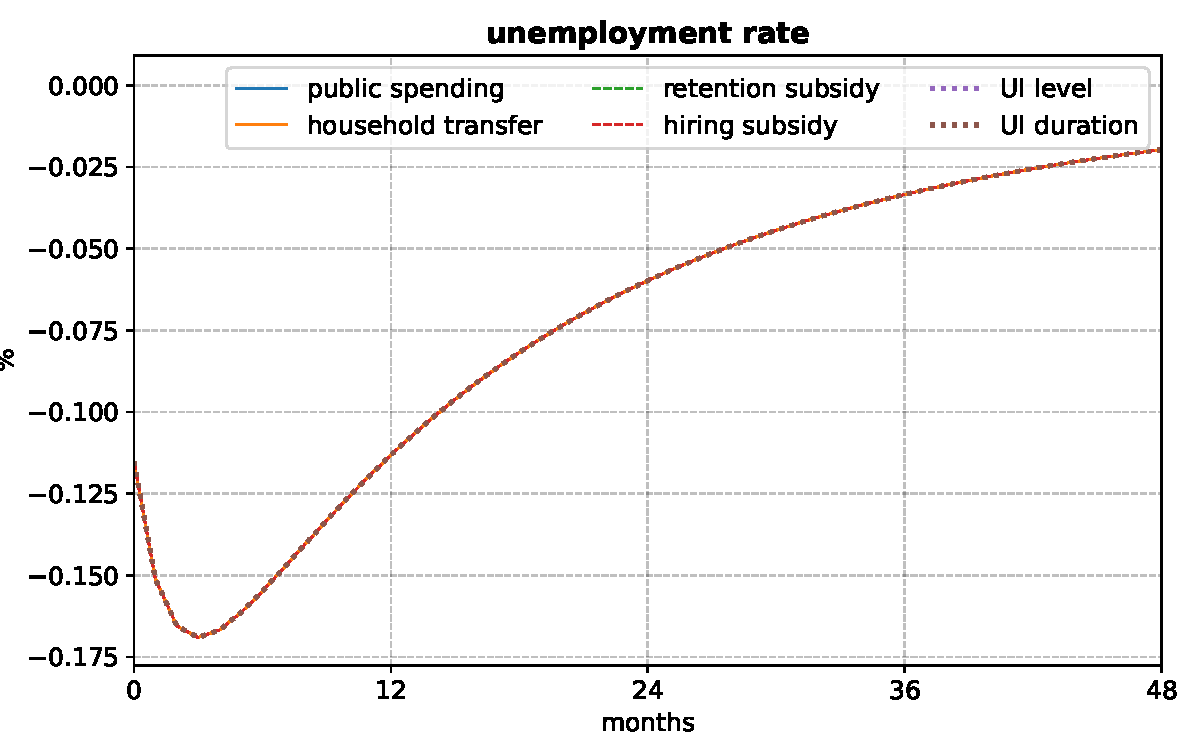
\includegraphics[scale=0.3]{results/pol_baseline_u_titled.pdf}
    \hfill
    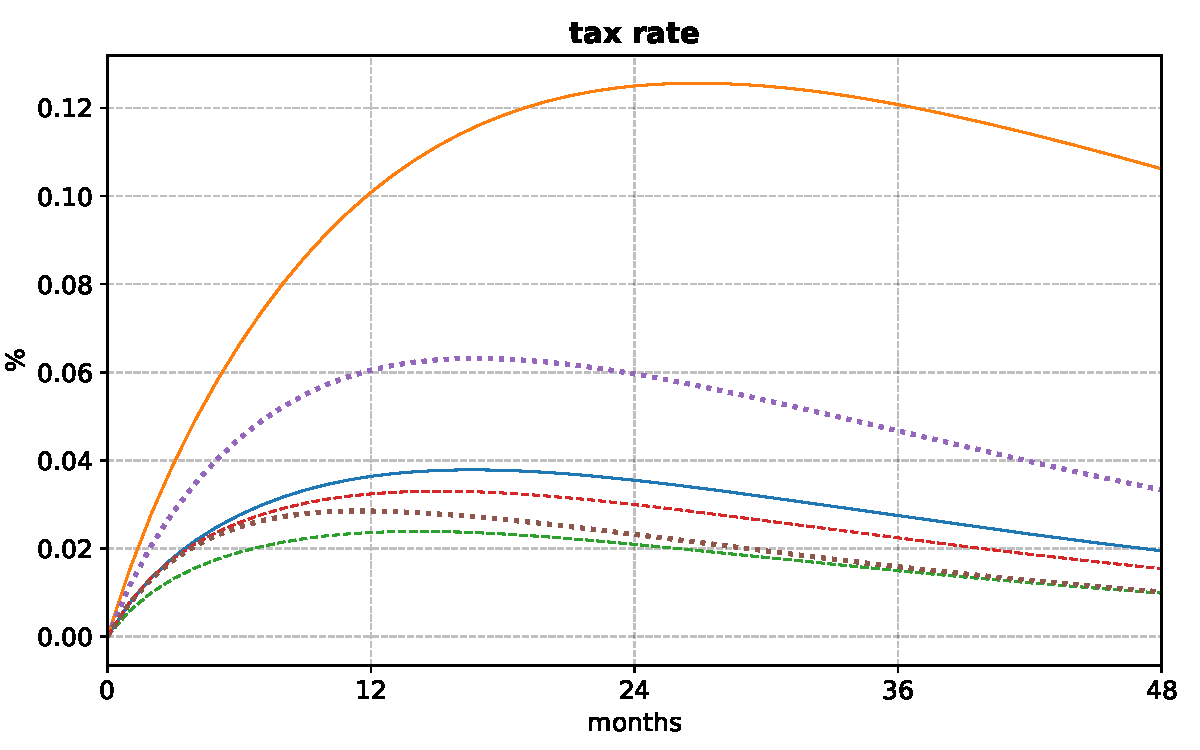
\includegraphics[scale=0.3]{results/pol_baseline_tau_titled.pdf}

    \begin{onlyenv}<1>
		\begin{itemize}
			\item Same unemployment path engineered with the six different policies
			\item Large variation in tax expenses $\leadsto$ large variation in fiscal multipliers
		\end{itemize}
    \end{onlyenv}
    \begin{onlyenv}<2>
        \begin{block}{Fiscal multipliers}
        \begin{center}
        \begin{tabular}{lllllll}
\multicolumn{1}{c}{}& \multicolumn{4}{c}{\textbf{HA/demand}} & \multicolumn{2}{c}{\textbf{SAM/supply}}\\
\toprule
 & \textbf{G} & \textbf{transfer}  & \textbf{UI level} & \textbf{UI duration} & \textbf{retention} & \textbf{hiring}\\
\midrule
baseline & 0.60 & 0.11  & 0.25 & 0.60 & 1.02 & 0.70\\
\bottomrule
\end{tabular}

        \end{center}
    \end{block}
    \end{onlyenv}
\end{frame}

\begin{frame}{Results: calibration matters, but cross-block dependence is small}

\begin{block}{Relative fiscal multipliers and the labor market}
        \begin{center}
            \begin{tabular}{lllllll}
\toprule
 & \textbf{G} & \textbf{transfer} & \textbf{retention} & \textbf{hiring} & \textbf{UI level} & \textbf{UI duration} \\
\midrule
baseline & 1.0 [0.60] & 0.19 & 1.72 & 1.17 & 0.41 & 1.00 \\
free entry & 1.0 [0.37] & 0.21 & 1.62 & 1.84 & 0.43 & 1.00 \\
exo. sep. & 1.0 [0.13] & 0.22 & 1.52 & 4.26 & 0.46 & 1.00 \\
\bottomrule
\end{tabular}

        \end{center}
    \end{block}

    \begin{itemize}
        \item Relative fiscal multipliers of demand-side policies insensitive to labor-market calibration
        \item Retention subsidies are powerful in our calibration since vacancy creation is inelastic and separations are elastic (compared to DMP)
    \end{itemize}
\end{frame}

\begin{frame}{Results: calibration matters, but cross-block dependence is small}
    
    \begin{block}{Relative fiscal multipliers and liquidity}
    \begin{center}
        \begin{tabular}{lllllll}
\multicolumn{1}{c}{}& \multicolumn{4}{c}{\textbf{HA/demand}} & \multicolumn{2}{c}{\textbf{SAM/supply}}\\
\toprule
 & \textbf{G} & \textbf{transfer}  & \textbf{UI level} & \textbf{UI duration} & \textbf{retention} & \textbf{hiring}\\
\midrule
baseline & 1.0 [0.60] & 0.19  & 0.41 & 1.00 & \color{gray}1.72 & \color{gray}1.17\\
$A/Y = 3.623$ & 1.0 [0.53] & 0.10  & 0.23 & 0.49 & \color{gray}1.77 & \color{gray}1.20\\
$A/Y = 1.228$ & 1.0 [0.73] & 0.33  & 0.71 & 2.06 & \color{gray}1.70 & \color{gray}1.16\\
\bottomrule
\end{tabular}

    \end{center}
    \end{block}

    \begin{itemize}
        \item Relative fiscal multipliers of supply-side policies insensitive to consumption-savings calibration
        \item With less liquidity, demand stimulus policies are more potent
        \item (not shown) More hand-to-mouth households \emph{lowers} fiscal multipliers (less response to risk)
    \end{itemize}

\end{frame}

\begin{frame}{Results: efficacy of firm-side policies depends on the MPC of capitalists}
    \begin{block}{Relative fiscal multipliers and firm ownership}
        \begin{center}
            \begin{tabular}{lllllll}
\multicolumn{1}{c}{}& \multicolumn{4}{c}{\textbf{HA/demand}} & \multicolumn{2}{c}{\textbf{SAM/supply}}\\
\toprule
 & \textbf{G} & \textbf{transfer}  & \textbf{UI level} & \textbf{UI duration} & \textbf{retention} & \textbf{hiring}\\
\midrule
baseline & 1.0 [0.60] & \color{gray}0.19  & \color{gray}0.41 & \color{gray}1.00 & 1.72 & 1.17\\
$0.5$ div. to PIH & 1.0 [0.56] & \color{gray}0.18  & \color{gray}0.40 & \color{gray}0.96 & 1.43 & 0.87\\
$0.5$ div. to PIH$\dagger$ & 1.0 [0.75] & \color{gray}0.18  & \color{gray}0.39 & \color{gray}1.00 & 1.56 & 0.76\\
\bottomrule
\end{tabular}

        \end{center}
        $\dagger$: recalibrated model
        \end{block}
    \begin{itemize}
        \item The efficacy of firm policies depends on the MPC of capitalists
        \item With dividends distributed to permanent-income households, the fiscal multipliers of firm subsidies are lower 
    \end{itemize}
\end{frame}

\section{Conclusion}

\begin{frame}{Conclusion}
    \begin{itemize}
        \item The fiscal multipliers for different fiscal policies depend on the entire structure of the economy\dots
        \item \dots but the comparison of demand-side policies is largely insensitive to assumptions on the supply side, and vice versa
        \item Retention subsidies are a potent policy in our framework
        \begin{itemize}
            \item Data: vacancies are ``sluggish'' $\Rightarrow$ better to target separations
        \end{itemize}
    \end{itemize}
\end{frame}

\appendix

\begin{frame}{Unemployment insurance}
\label{slide:ui}
	US-style duration-dependent UI system:

\begin{itemize}
\item High replacement rate, 0.76, first 6 months
\item Low replacement rate, 0.55, 
after 6 months
\item With probability $0.52$, households receive
low UI immediately
\end{itemize}

(matching household income during unemployment spell, and share of unemployed with unemployment benefits)

\hyperlink{slide:calibration}{\beamerbutton{back}}


\end{frame}

\begin{frame}{Consumption upon unemployment}
\label{slide:preferences}

\begin{itemize}
\item \textbf{Stylized fact \#1: }Consumption $\approx$ 20\% lower
for unemployed (Chodorow-Reich-Karabarbounis, 2016)
\item \textbf{Stylized fact \#2: }Drop at UI exhaustion of $\approx$ 45\%
of income drop (Ganong-Noel, 2019)
\end{itemize}
\begin{center}
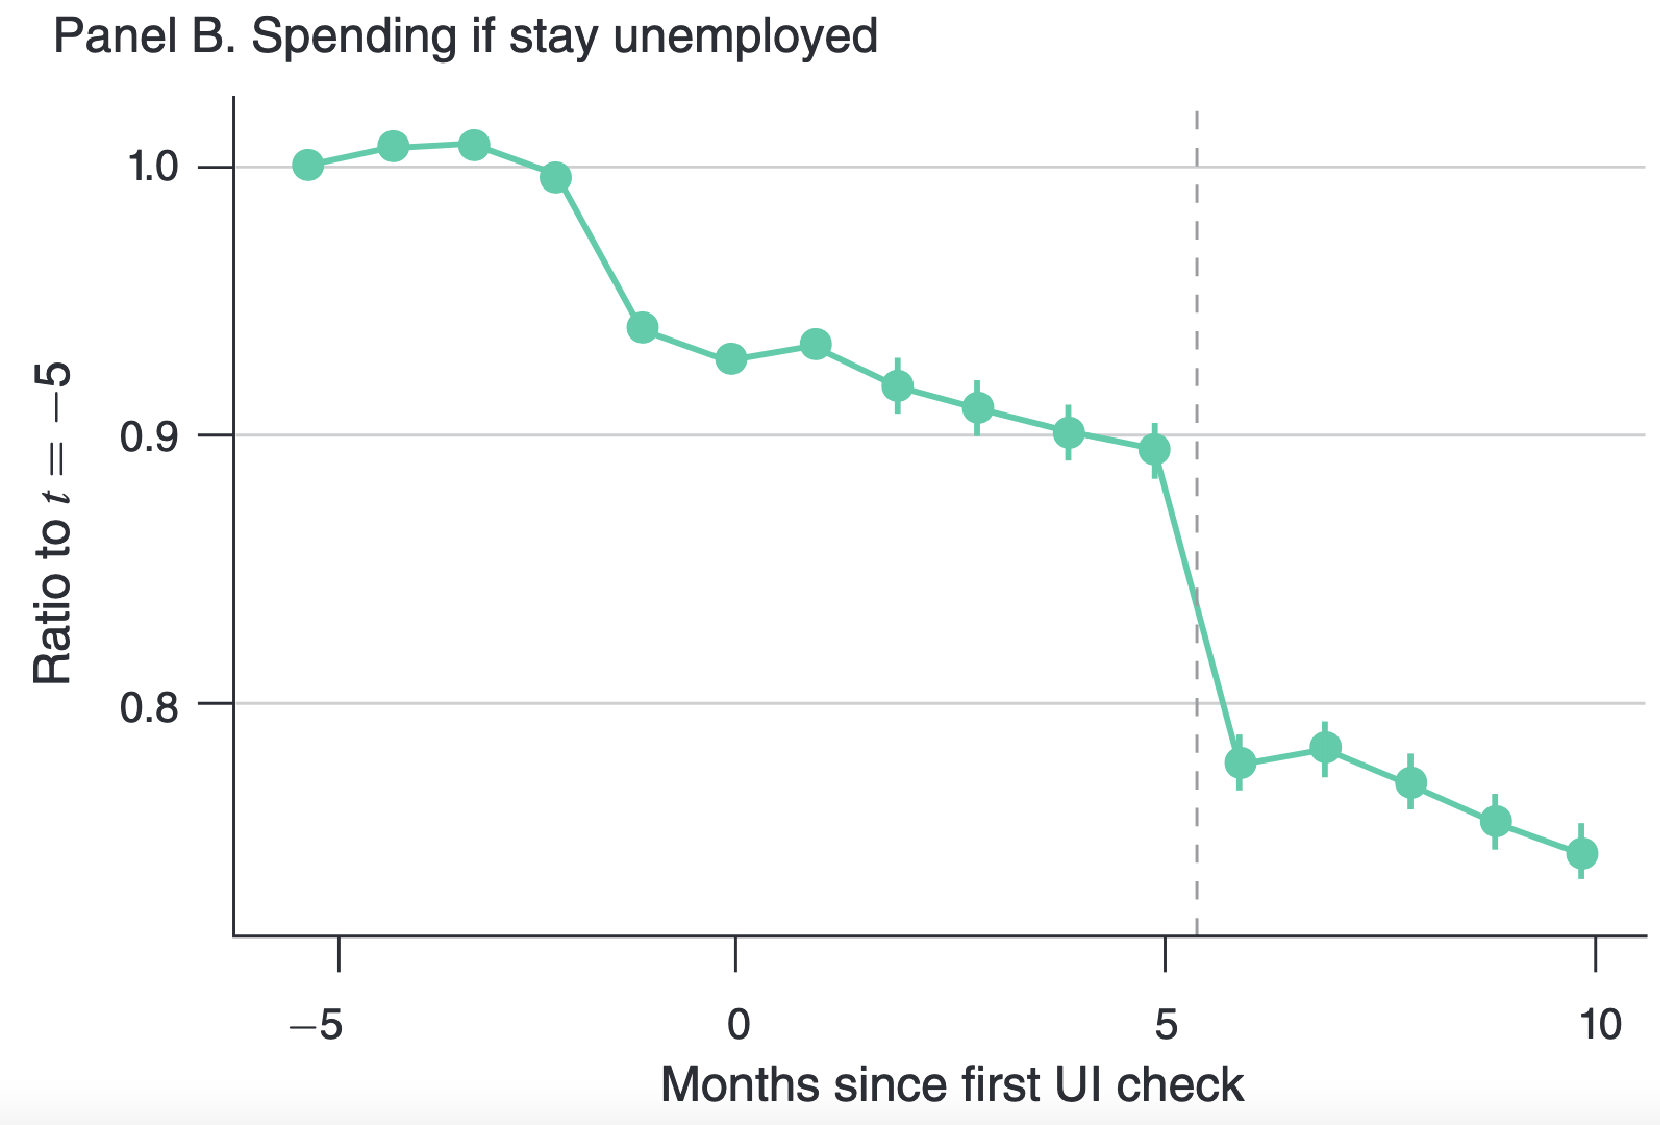
\includegraphics[width=0.35\linewidth]{figs/Ganong19}
\par\end{center}

\begin{center}
\vspace{-3mm}\textbf{\footnotesize{}Source:}{\footnotesize{} Ganong-Noel
(2019)}{\footnotesize\par}
\par\end{center}
\hyperlink{slide:calibration}{\beamerbutton{back}}
\end{frame}

\begin{frame}{Household preferences and consumption upon unemployment}

\begin{enumerate}
\item \textbf{Share of HtM households}: Consumption drop at expiration of
UI
\item \textbf{Discount factor}, $\beta$: Consumption drop during unemployment
\end{enumerate}
\begin{center}
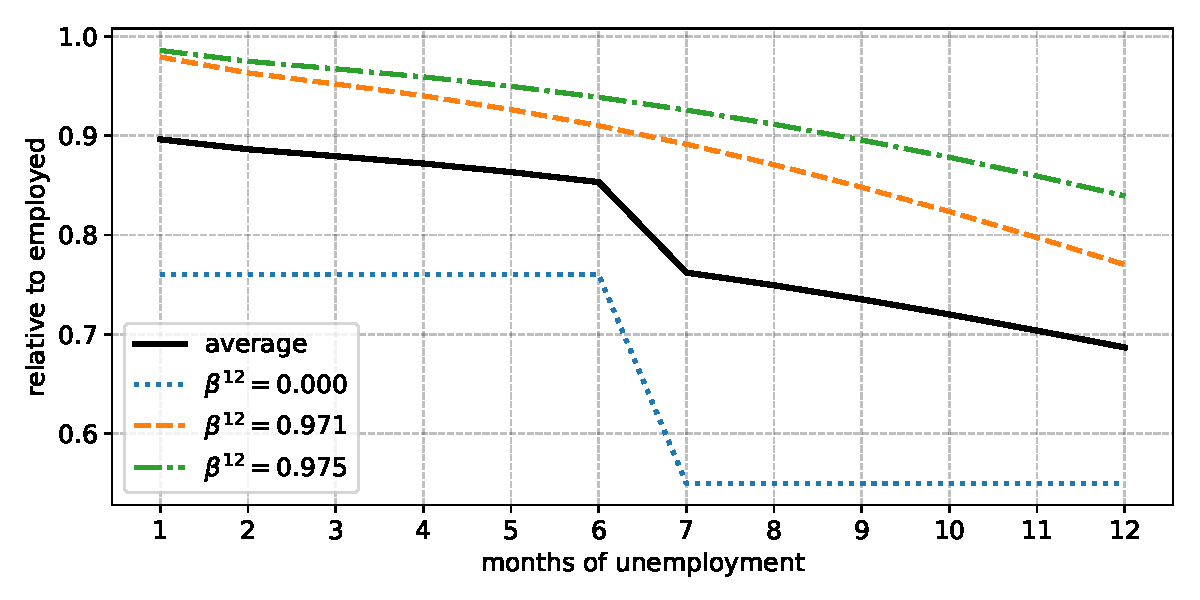
\includegraphics[width=0.8\linewidth]{results/c_upon_u}
\par\end{center}

\vspace{-4mm}\textbf{Note:} Calibration implies quarterly MPC at
41 \%
(in line with Johnson-Parker-Souleles, 2001). \hyperlink{slide:calibration}{\beamerbutton{back}}

\end{frame}

\begin{frame}{Relative job-finding rates}
\label{slide:rel_job_finding}

\begin{center}
\textbf{Job-finding rate relative to first month in unemployment:}

	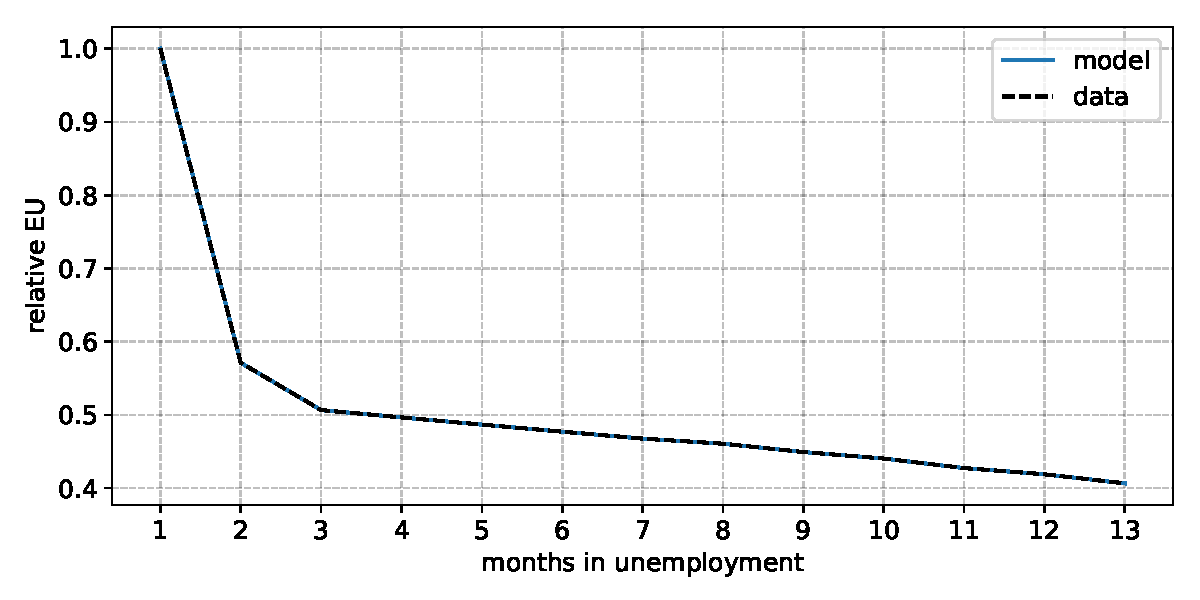
\includegraphics[width=0.9\linewidth]{results/UEs}
\end{center}

\hyperlink{slide:calibration}{\beamerbutton{back}}
\end{frame}

\begin{frame}{Separation rate leads job-finding rate}
\label{slide:dyn_job_finding_seprations}

\begin{center}
\begin{tabular}{cc}
\textbf{Monetary policy shock} & \textbf{Technology shock}\tabularnewline
\textbf{\small{}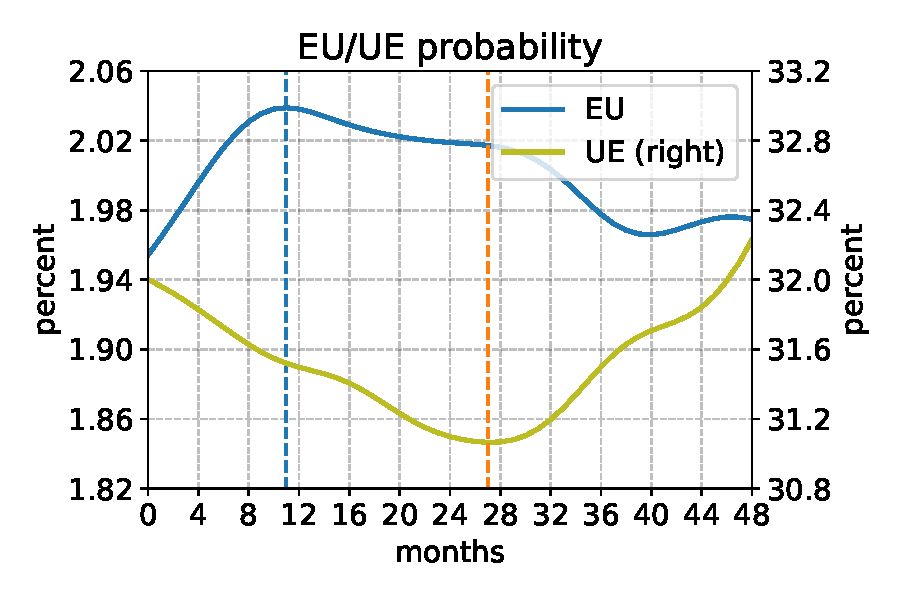
\includegraphics[width=0.45\textwidth]{results/monetary_shock_lead_lag}} & \textbf{\small{}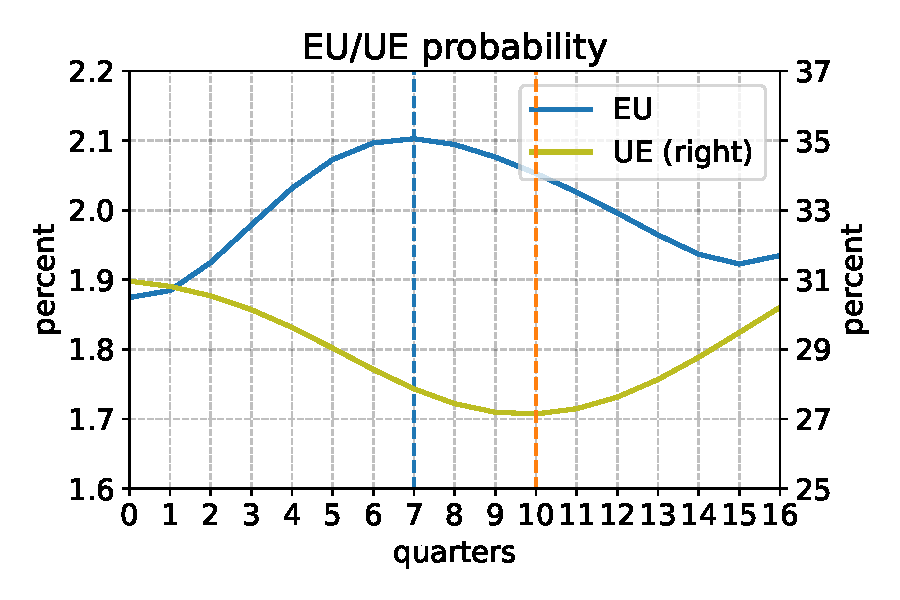
\includegraphics[width=0.45\textwidth]{results/technology_shock_lead_lag}}\tabularnewline
\end{tabular}

\textbf{\footnotesize{}Source: }{\footnotesize{}CPS 1967-2020; Romer-Romer
MP shock; Fernald TFP shock}.\vspace{3mm}
\end{center}




\textbf{Stylized Fact \#3:} \emph{Separation rate leads job-finding rate by 9-16 months.}
\end{frame}

\begin{frame}{Separation rate accounts for substantial share of unemployment}

\begin{center}

\begin{tabular}{cc}
\textbf{Monetary policy shock} & \textbf{TFP shock}\tabularnewline
\textbf{\small{}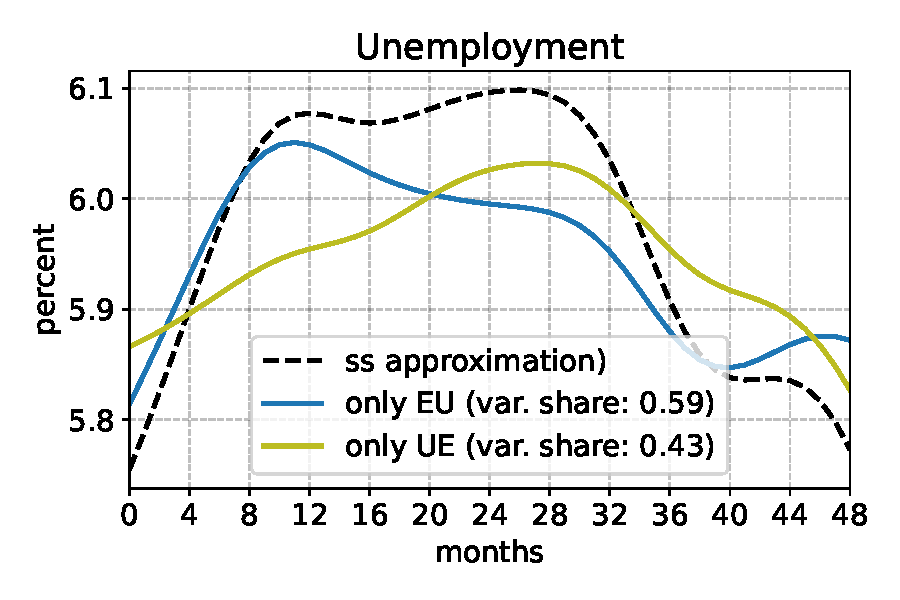
\includegraphics[width=0.45\textwidth]{results/monetary_shock_decomposition}} & \textbf{\small{}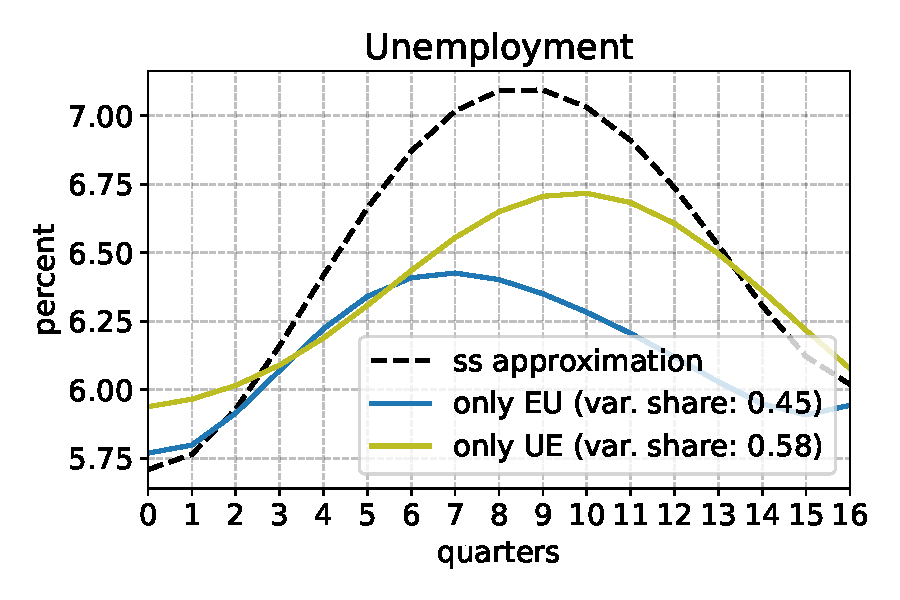
\includegraphics[width=0.45\textwidth]{results/technology_shock_decomposition}}\tabularnewline
\end{tabular}

\textbf{\footnotesize{}Source: }{\footnotesize{}CPS 1967-2020; Romer-Romer
MP shock; Fernald TFP shock}.\vspace{3mm}

\end{center}
\textbf{Stylized Fact \#4:} \emph{Separations account for 40-60 percent of unemployment response.}
\hyperlink{slide:calibration}{\beamerbutton{back}}

\end{frame}

\end{document}